\section{Nano}
\begin{frame}
\begin{center}
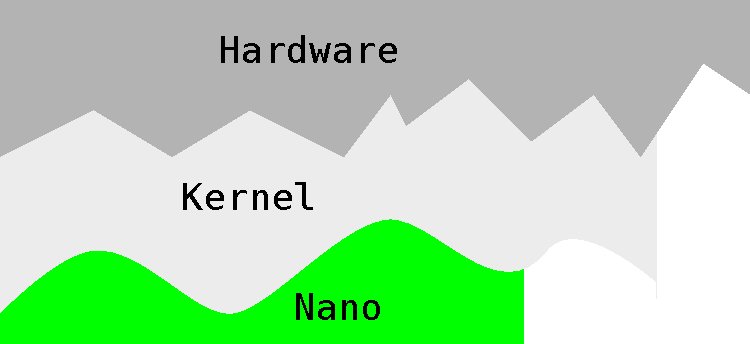
\includegraphics[width=0.5\textwidth]{nano.pdf}
\end{center}
\begin{itemize}
 \item \cod{config/Makefile}
 \item \cod{src/s-nano.S}
 \begin{description}
  \item[target-root] nichts
 \end{description}
 \item \cod{src/c-nano.c}
 \begin{description}
  \item[target-root] \cod{libc.a} wegen \cod{syscall}
 \end{description}
\end{itemize}
\end{frame}
